\documentclass[]{IEEEtran}
% some very useful LaTeX packages include:
%\usepackage{cite}      
\usepackage{graphicx}   
\usepackage{subfigure} 
\usepackage{url}       
\usepackage{amsmath}    
\usepackage{caption2}
% Your document starts here!
\begin{document}

% Define document title and author
	\title{Weekly Report}
	\author{Adviser: Prof. Yang Wen \\Student: Cheng Wensheng\\ Period: 2018.5.18-5.25
	}
	\markboth{Visual Information Processing Group}{}
	\maketitle

% Write abstract here
\begin{abstract}
	This week I mainly put my effort on keeping finding materials of SAR image contest and reading a new paper about pooling, which is accepted by CVPR 2018 as oral paper. 
\end{abstract}

% Each section begins with a \section{title} command
\section{Paper reading}
	% \PARstart{}{} creates a tall first letter for this first paragraph
	\PARstart{I}{n} this paper, they aim to leverage recent results on image downscaling for the purposes of deep learning. Inspired by the human visual system, which focuses on local spatial changes, they propose \textbf{detail preserving pooling (DPP)}, an adaptive pooling method that magnifies spatial changes and preserves important structural detail. Importantly, its parameters can be learned jointly with the rest of the network. They analyze some of its theoretical properties and show its empirical benefits on several datasets and networks, where DPP consistently outperforms previous pooling approaches. Overall, the contributions are as follows:
	\begin{itemize}
		\item They presented a novel pooling layer for convolutional neural networks termed detail-preserving pooling (DPP), based on the idea of inverse bilateral filters.
		\item DPP allows downscaling to focus on important structural detail; learnable parameters control the amount of detail preservation.
		\item DPP can be combined with stochastic pooling methods
		with further accuracy gains as detail preservation and
		regularization complement each other.
	\end{itemize}

	The author showed theoretically that DPP can adapt to perform similar	to max/extremum or average pooling, or on a nonlinear
	continuum of intermediate functions while incurring only
	a minor computational overhead. I think it might be useful for my semantic segmentation work. Fig.~\ref{fig:mp} is the Diagram of detail-preserving downscaling (DPID) and detail-preserving pooling (DPP). Fig.~\ref{fig:ss} is the downscaling visual comparison with other methods.
	

% Main Part

\newpage
\begin{figure}[!hbt]
%		 Center the figure.
		\vspace{1.7cm}
%		\hspace{50cm}
		\begin{center}
			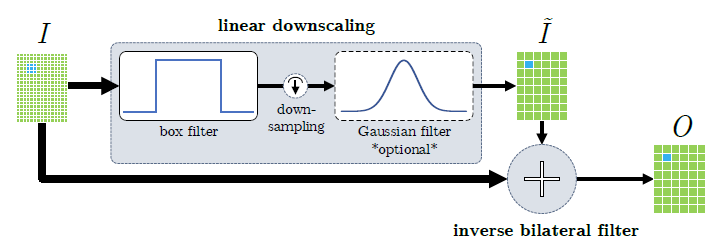
\includegraphics[width=\columnwidth]{t1}
				%		 Create a subtitle for the figure.
			\caption{Diagram of DPP and DPP}
			\label{fig:mp}
		    \hspace{0.5cm}
			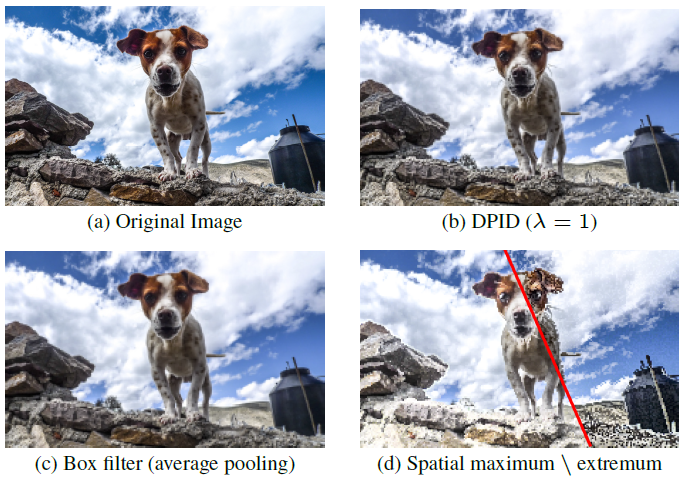
\includegraphics[width=\columnwidth]{t2}
				%Create a subtitle for the figure.
			\caption{Downscaling visual comparison}
			\label{fig:ss}
		\end{center}
	\end{figure}

% Now we need a bibliography:
%\begin{thebibliography}{5}
%
%	%Each item starts with a \bibitem{reference} command and the details thereafter.
%	\bibitem{HOP96} % Transaction paper
%	J.~Hagenauer, E.~Offer, and L.~Papke. Iterative decoding of binary block
%	and convolutional codes. {\em IEEE Trans. Inform. Theory},
%	vol.~42, no.~2, pp.~429–-445, Mar. 1996.
%
%	\bibitem{MJH06} % Conference paper
%	T.~Mayer, H.~Jenkac, and J.~Hagenauer. Turbo base-station cooperation for intercell interference cancellation. {\em IEEE Int. Conf. Commun. (ICC)}, Istanbul, Turkey, pp.~356--361, June 2006.
%
%	\bibitem{Proakis} % Book
%	J.~G.~Proakis. {\em Digital Communications}. McGraw-Hill Book Co.,
%	New York, USA, 3rd edition, 1995.
%
%	\bibitem{talk} % Web document
%	F.~R.~Kschischang. Giving a talk: Guidelines for the Preparation and Presentation of Technical Seminars.
%	\url{http://www.comm.toronto.edu/frank/guide/guide.pdf}.
%
%	\bibitem{5}
%	IEEE Transactions \LaTeX and Microsoft Word Style Files.
%	\url{http://www.ieee.org/web/publications/authors/transjnl/index.html}
%
%\end{thebibliography}

% Your document ends here!
\end{document}